\chapter{Rechenzeit Daten}
\label{ch:performance_data}

\begin{figure}[H]
    \centering
    
\includegraphics[width=\linewidth]{evaluation/report/performance/complexPositionWithManyOptions/ComplexPositionWithManyOptions}
    \caption{ComplexPositionWithManyOptions - logarithmische Skala}
    \label{fig:ComplexPositionWithManyOptions}
\end{figure}

\begin{figure}[H]
    \centering
    
\includegraphics[width=\linewidth]{evaluation/report/performance/complexTacticalMiddleGame/ComplexTacticalMiddleGame}
    \caption{ComplexTacticalMiddleGame - logarithmische Skala}
    \label{fig:ComplexTacticalMiddleGame}
\end{figure}

\begin{figure}[H]
    \centering
    
\includegraphics[width=\linewidth]{evaluation/report/performance/endGameDeflectionShort/EndGame-Deflection-Short}
    \caption{EndGameDeflectionShort - logarithmische Skala}
    \label{fig:EndGameDeflectionShort}
\end{figure}

\begin{figure}[H]
    \centering
    
\includegraphics[width=\linewidth]{evaluation/report/performance/forkOpportunity/ForkOpportunity}
    \caption{ForkOpportunity - logarithmische Skala}
    \label{fig:ForkOpportunity}
\end{figure}

\begin{figure}[H]
    \centering
    
\includegraphics[width=\linewidth]{evaluation/report/performance/midGameDeflectionShort/MidGame-Deflection-Short}
    \caption{MidGameDeflectionShort - logarithmische Skala}
    \label{fig:MidGameDeflectionShort}
\end{figure}

\begin{figure}[H]
    \centering
    
\includegraphics[width=\linewidth]{evaluation/report/performance/midGameDiscoveryMateIn2Short/MidGame-Discovery-MateIn2-Short}
    \caption{MidGameDiscoveryMateIn2Short - logarithmische Skala}
    \label{fig:MidGameDiscoveryMateIn2Short}
\end{figure}

\begin{figure}[H]
    \centering
    
\includegraphics[width=\linewidth]{evaluation/report/performance/midGameDiscoveryShort/MidGame-Discovery-Short}
    \caption{MidGameDiscoveryShort - logarithmische Skala}
    \label{fig:MidGameDiscoveryShort}
\end{figure}

\begin{figure}[H]
    \centering
    
\includegraphics[width=\linewidth]{evaluation/report/performance/midGameEnPassantLong/MidGame-EnPassant-Long}
    \caption{MidGameEnPassantLong - logarithmische Skala}
    \label{fig:MidGameEnPassantLong}
\end{figure}

\begin{figure}[H]
    \centering
    
\includegraphics[width=\linewidth]{evaluation/report/performance/midGameForkShort/MidGame-Fork-Short}
    \caption{MidGameForkShort - logarithmische Skala}
    \label{fig:MidGameForkShort}
\end{figure}

\begin{figure}[H]
    \centering
    
\includegraphics[width=\linewidth]{evaluation/report/performance/midGamePromotionMateIn2Short/MidGame-Promotion-MateIn2-Short}
    \caption{MidGamePromotionMateIn2Short - logarithmische Skala}
    \label{fig:MidGamePromotionMateIn2Short}
\end{figure}

\begin{figure}[H]
    \centering
    
\includegraphics[width=\linewidth]{evaluation/report/performance/midgameTacticalCluster/MidgameTacticalCluster}
    \caption{MidgameTacticalCluster - logarithmische Skala}
    \label{fig:MidgameTacticalCluster}
\end{figure}

\begin{figure}[H]
    \centering
    
\includegraphics[width=\linewidth]{evaluation/report/performance/simpleTacticalPosition/SimpleTacticalPosition}
    \caption{SimpleTacticalPosition - logarithmische Skala}
    \label{fig:SimpleTacticalPosition}
\end{figure}

\section{Mittlere absolute Abweichungen vom Median}
\label{sec:mad}
\subfile{evaluation/report/performance/complexPositionWithManyOptions/ComplexPositionWithManyOptions-deviation}
\newpage
\subfile{evaluation/report/performance/complexTacticalMiddleGame/ComplexTacticalMiddleGame-deviation}
\newpage
\subfile{evaluation/report/performance/endGameDeflectionShort/EndGame-Deflection-Short-deviation}
\newpage
\subfile{evaluation/report/performance/forkOpportunity/ForkOpportunity-deviation}
\newpage
\subfile{evaluation/report/performance/midGameDeflectionShort/MidGame-Deflection-Short-deviation}
\newpage
\subfile{evaluation/report/performance/midGameDiscoveryMateIn2Short/MidGame-Discovery-MateIn2-Short-deviation}
\newpage
\subfile{evaluation/report/performance/midGameDiscoveryShort/MidGame-Discovery-Short-deviation}
\newpage
\subfile{evaluation/report/performance/midGameEnPassantLong/MidGame-EnPassant-Long-deviation}
\newpage
\subfile{evaluation/report/performance/midGameForkShort/MidGame-Fork-Short-deviation}
\newpage
\subfile{evaluation/report/performance/midGamePromotionMateIn2Short/MidGame-Promotion-MateIn2-Short-deviation}
\newpage
\subfile{evaluation/report/performance/midgameTacticalCluster/MidgameTacticalCluster-deviation}
\newpage
\subfile{evaluation/report/performance/simpleTacticalPosition/SimpleTacticalPosition-deviation}
\newpage

\section{Rechenzeiten pro Zugtiefe}
\label{sec:rechenzeiten-pro-zugtiefe}

\begin{figure}[H]
    \centering
    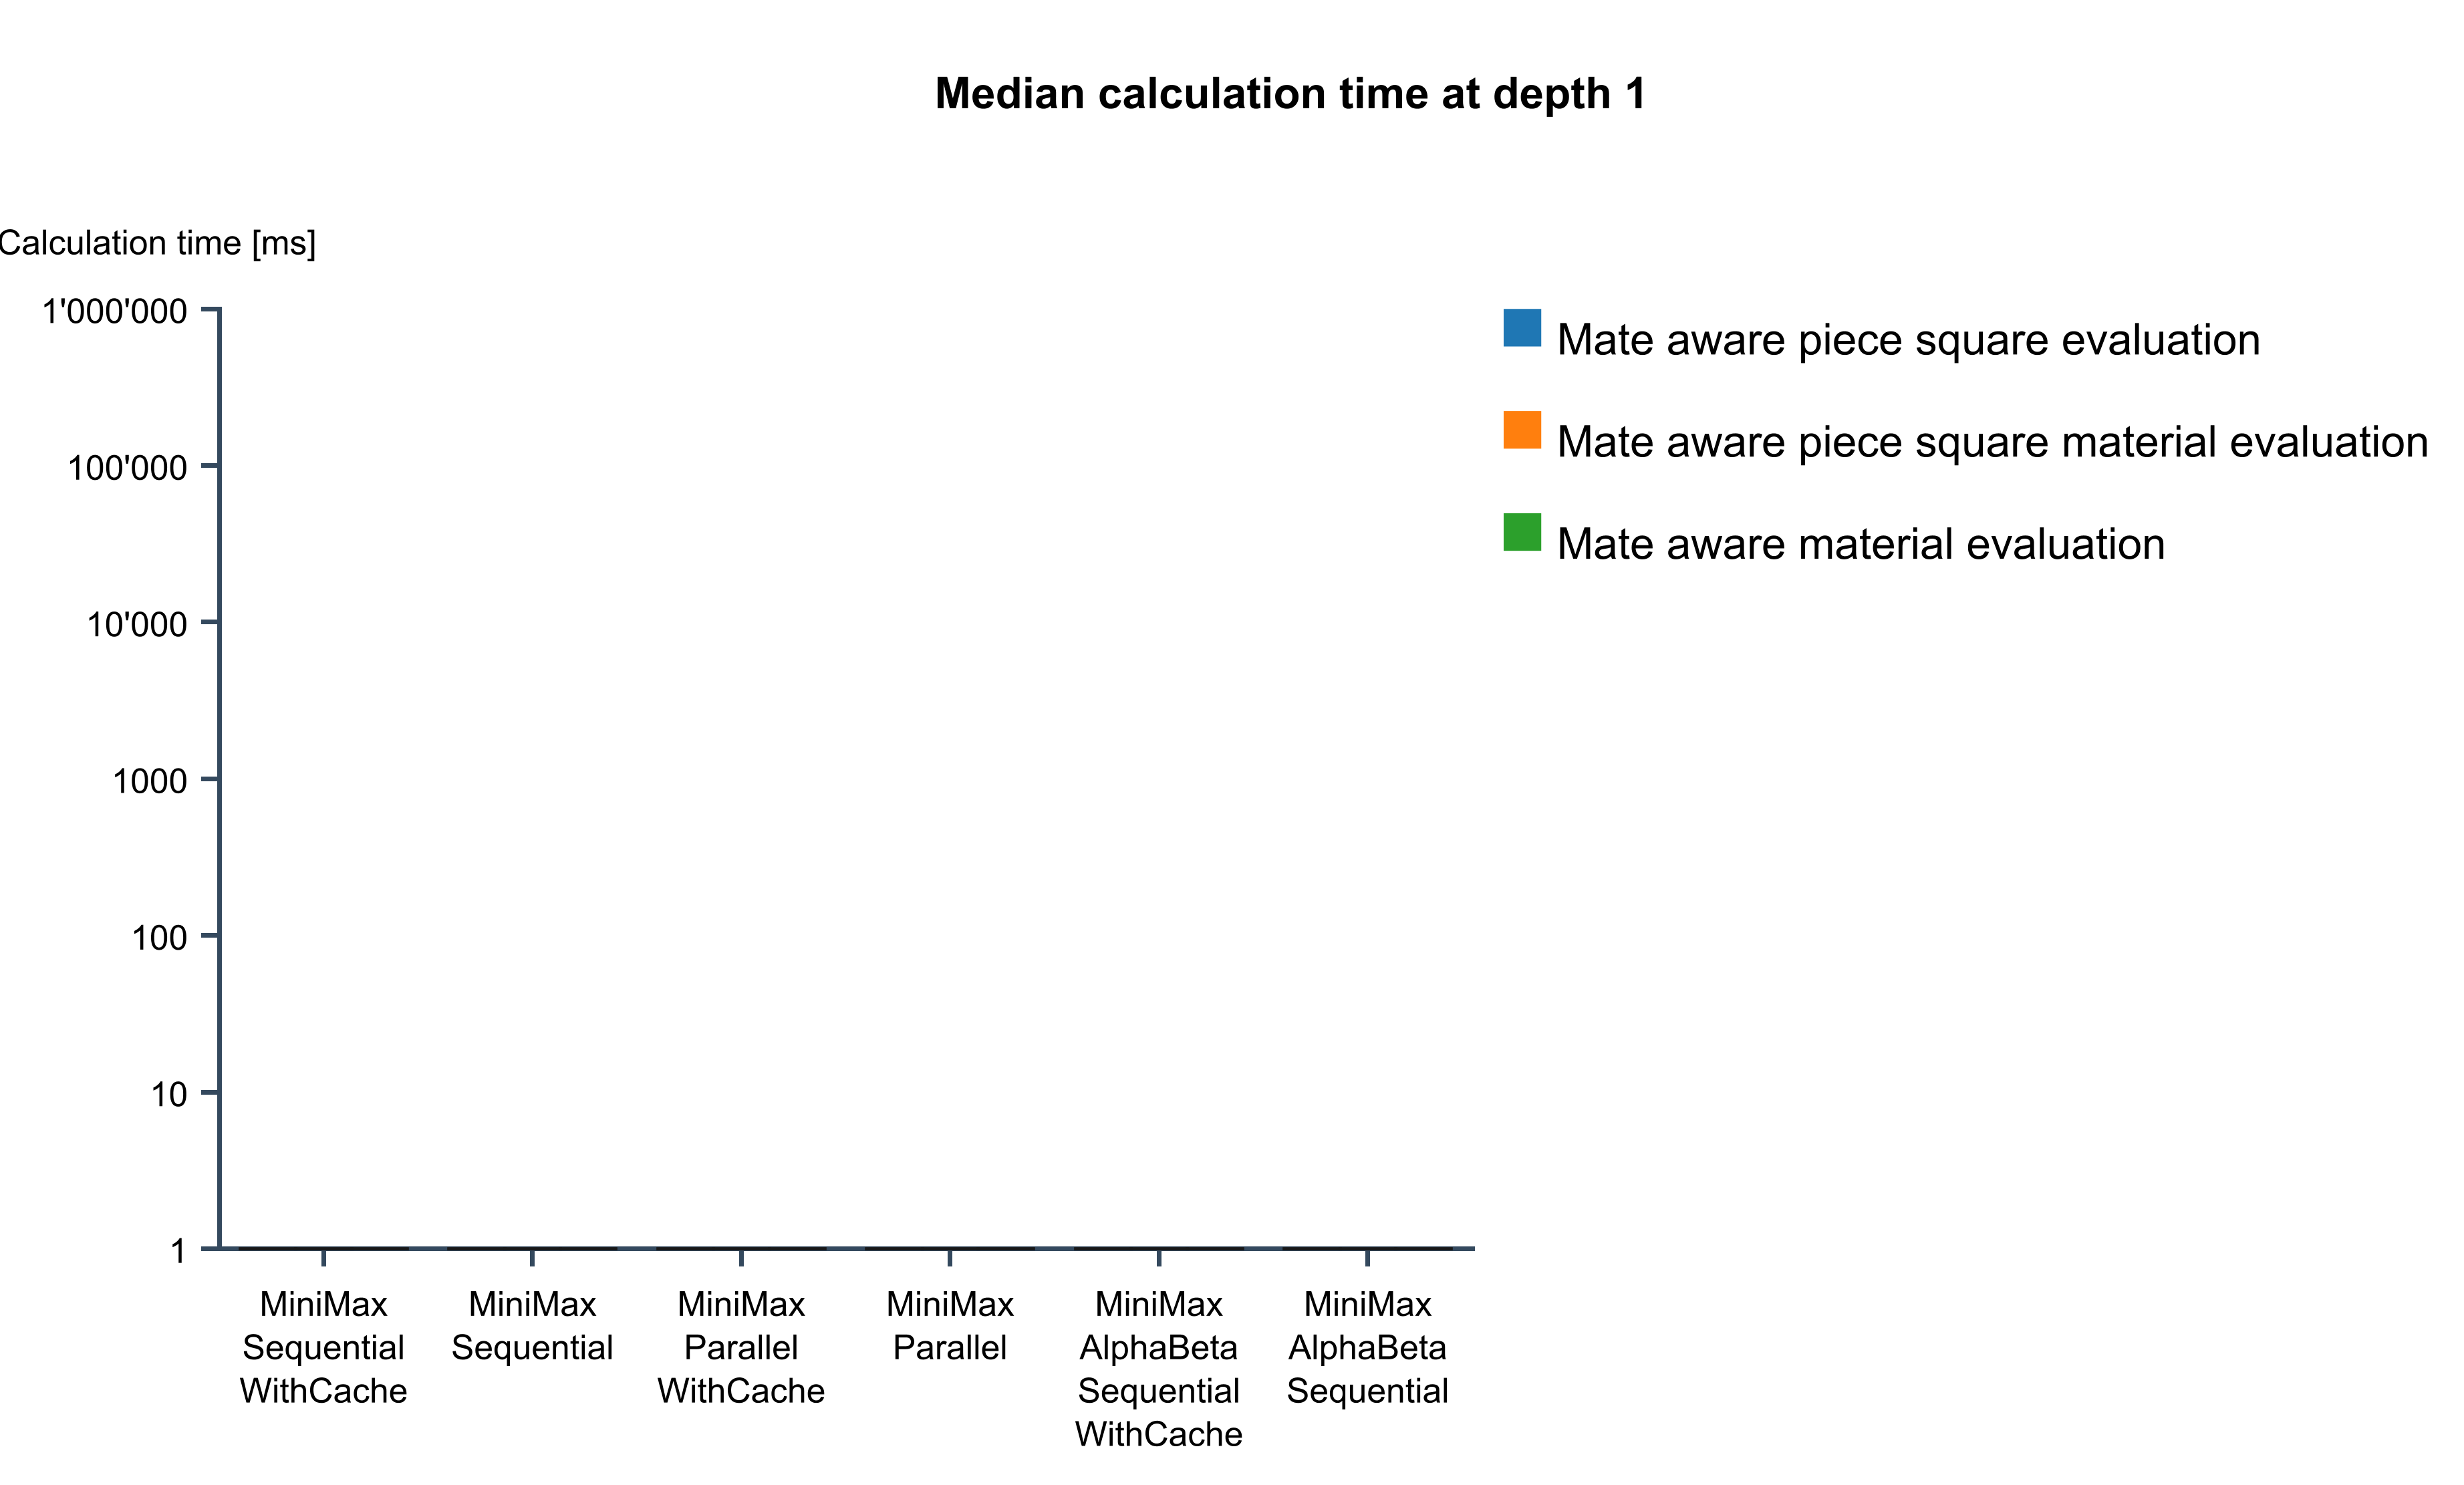
\includegraphics[width=\linewidth]{evaluation/report/performance/performance-at-depth-1-by-strategy}
    \caption{Rechenzeit für Zugtiefe 1}
    \label{fig:rechenzeit-fuer-tiefe-1}
\end{figure}

\begin{figure}[H]
    \centering
    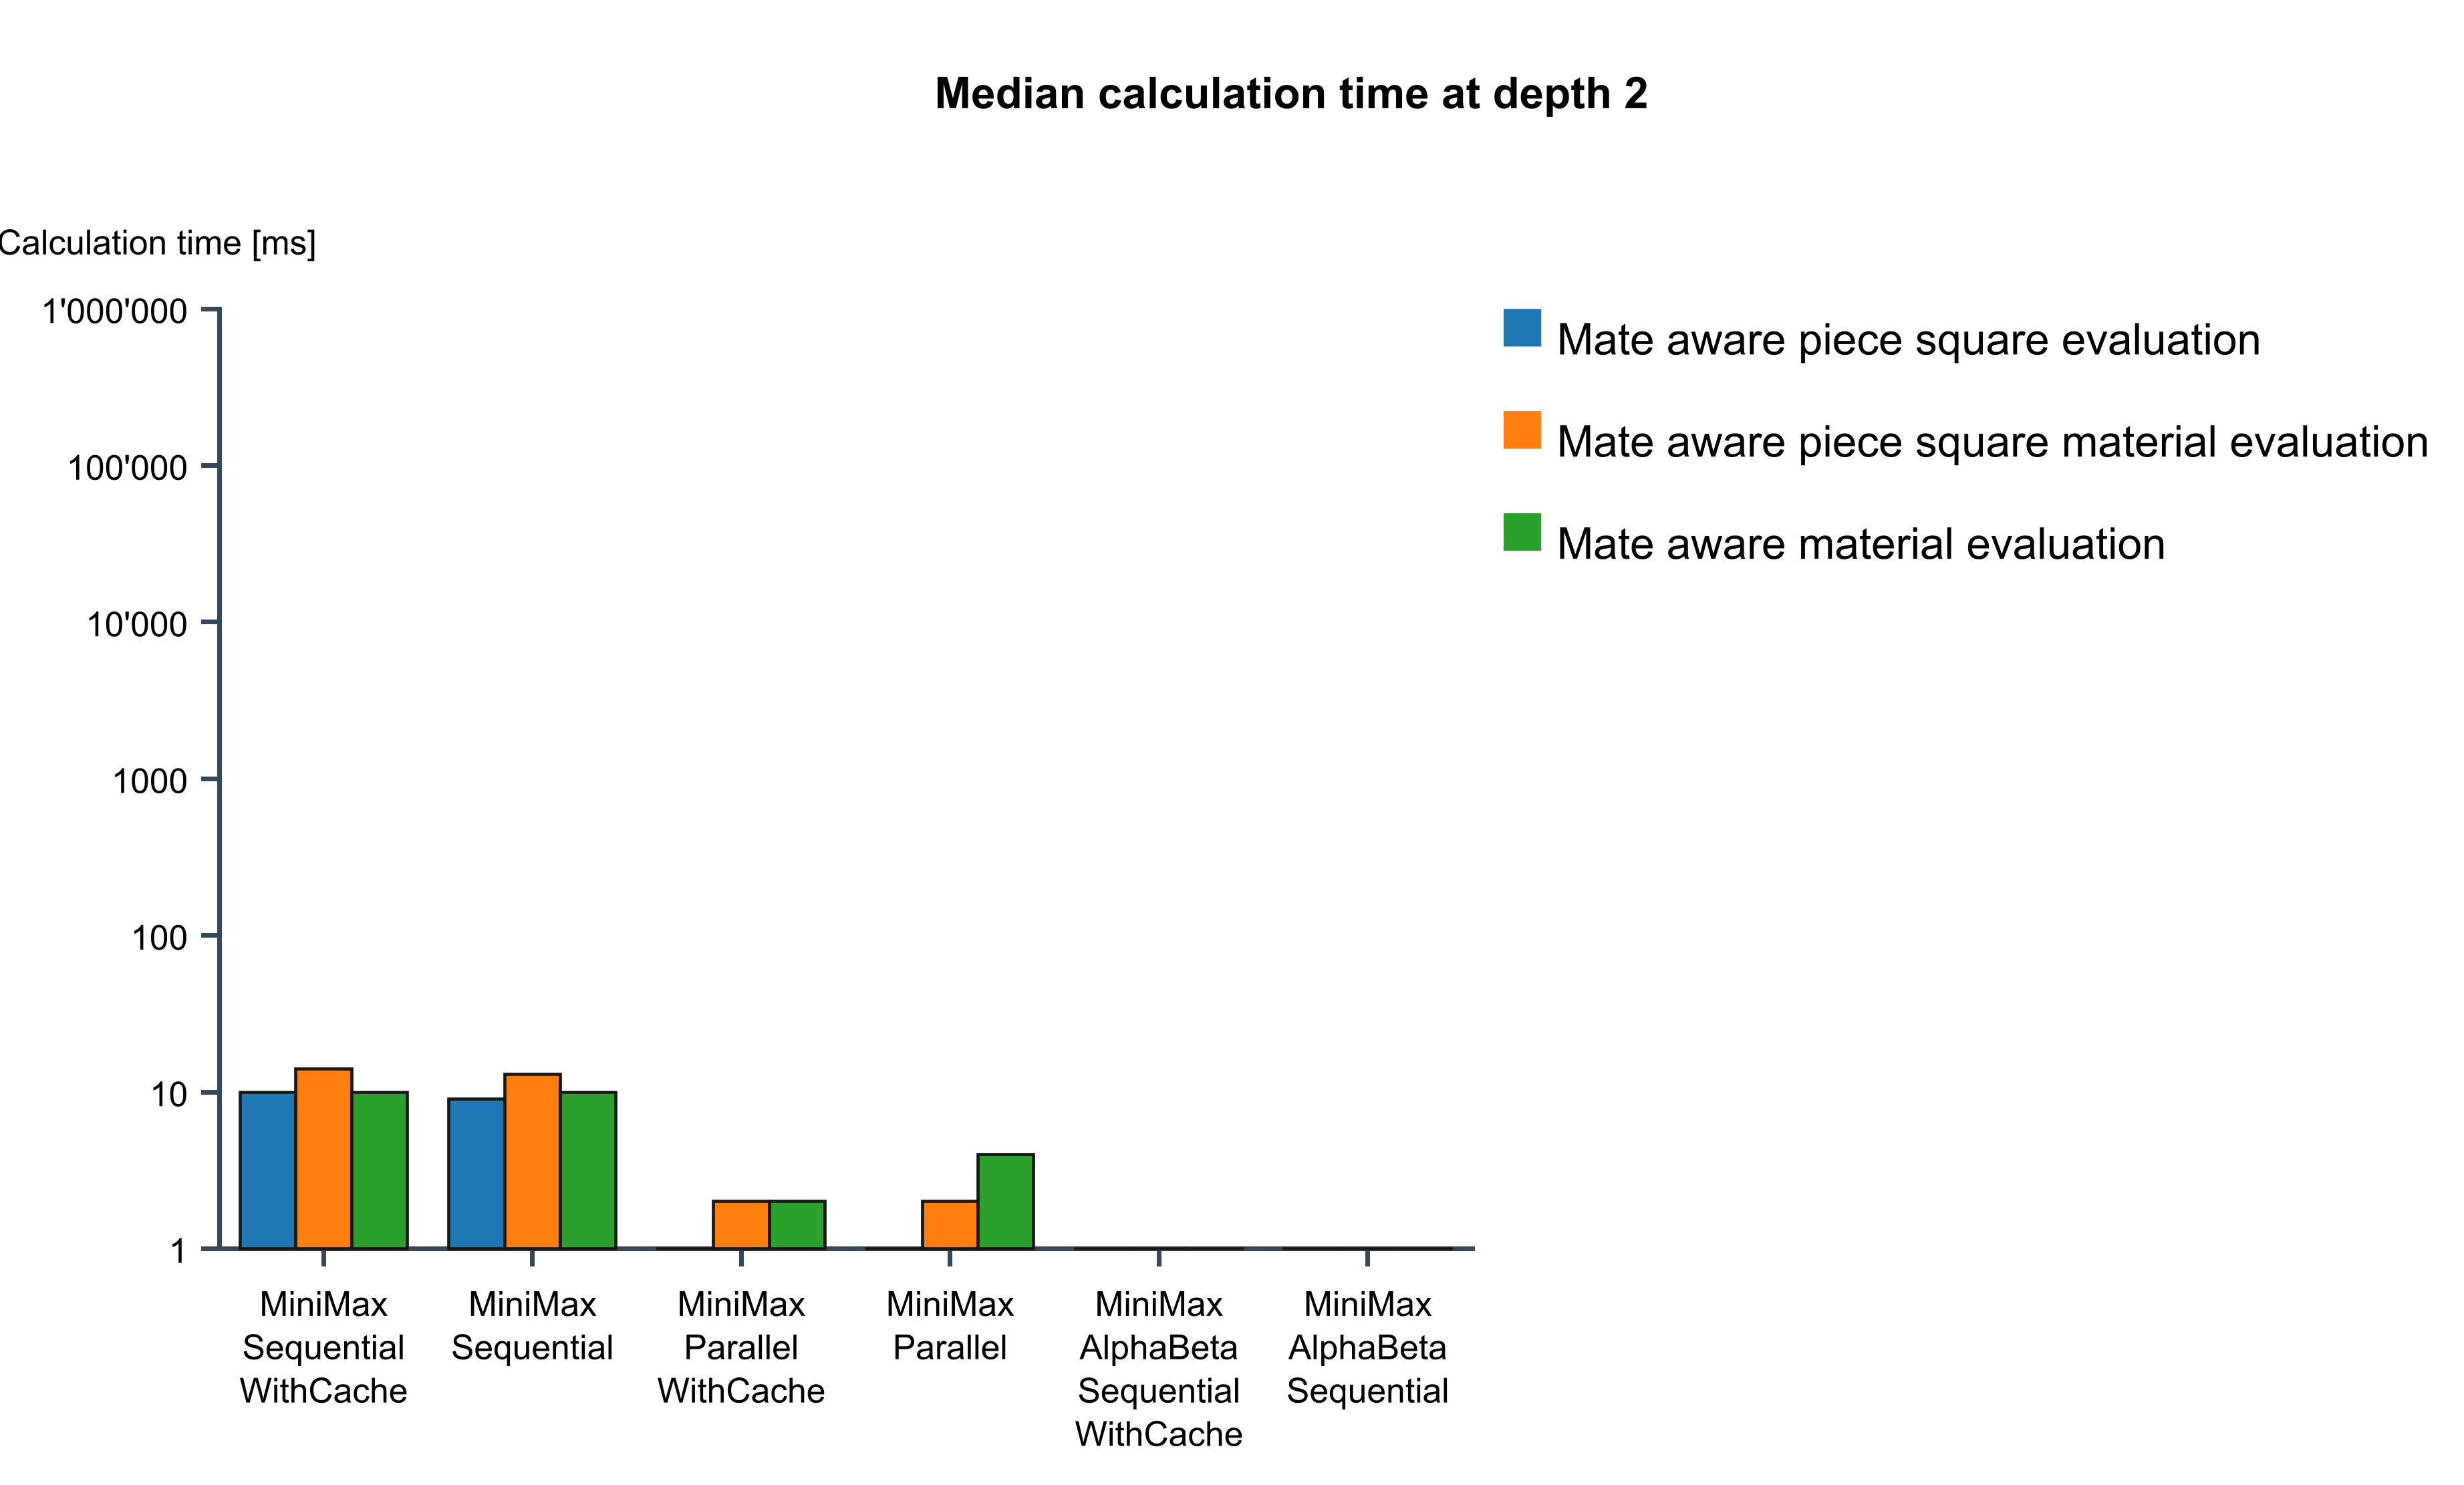
\includegraphics[width=\linewidth]{evaluation/report/performance/performance-at-depth-2-by-strategy}
    \caption{Rechenzeit für Zugtiefe 2}
    \label{fig:rechenzeit-fuer-tiefe-2}
\end{figure}

\begin{figure}[H]
    \centering
    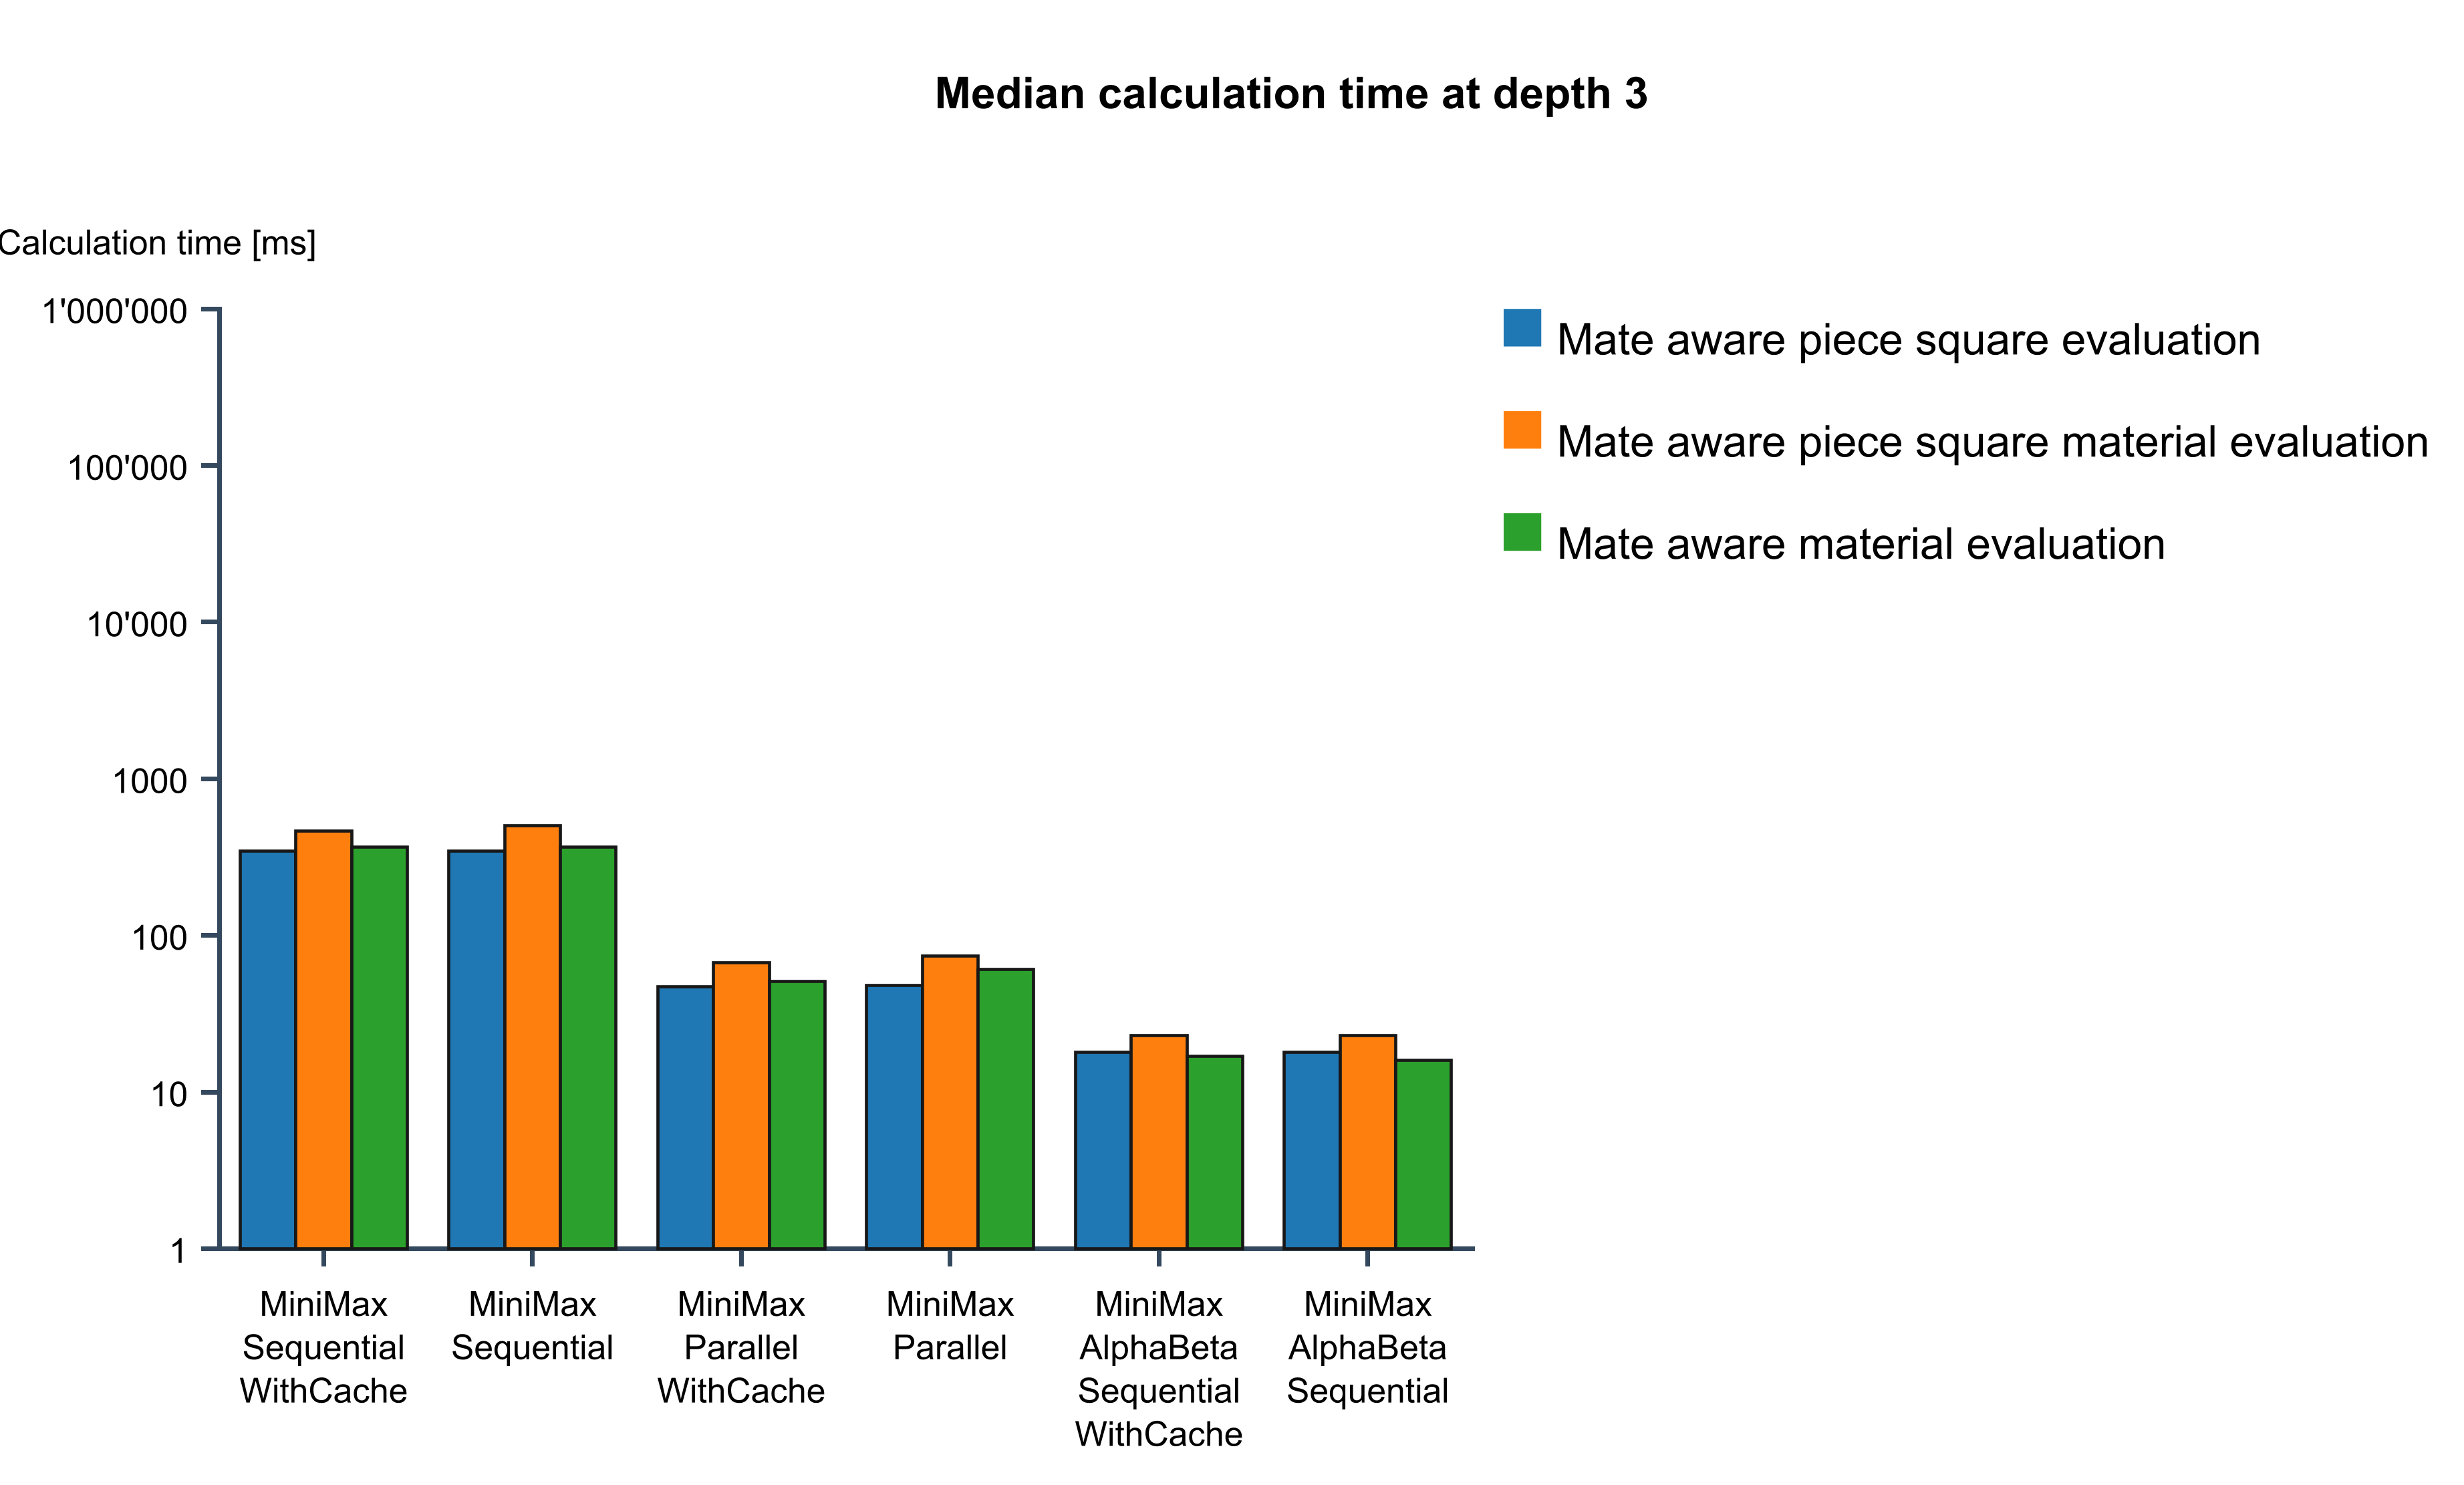
\includegraphics[width=\linewidth]{evaluation/report/performance/performance-at-depth-3-by-strategy}
    \caption{Rechenzeit für Zugtiefe 3}
    \label{fig:rechenzeit-fuer-tiefe-3}
\end{figure}

\begin{figure}[H]
    \centering
    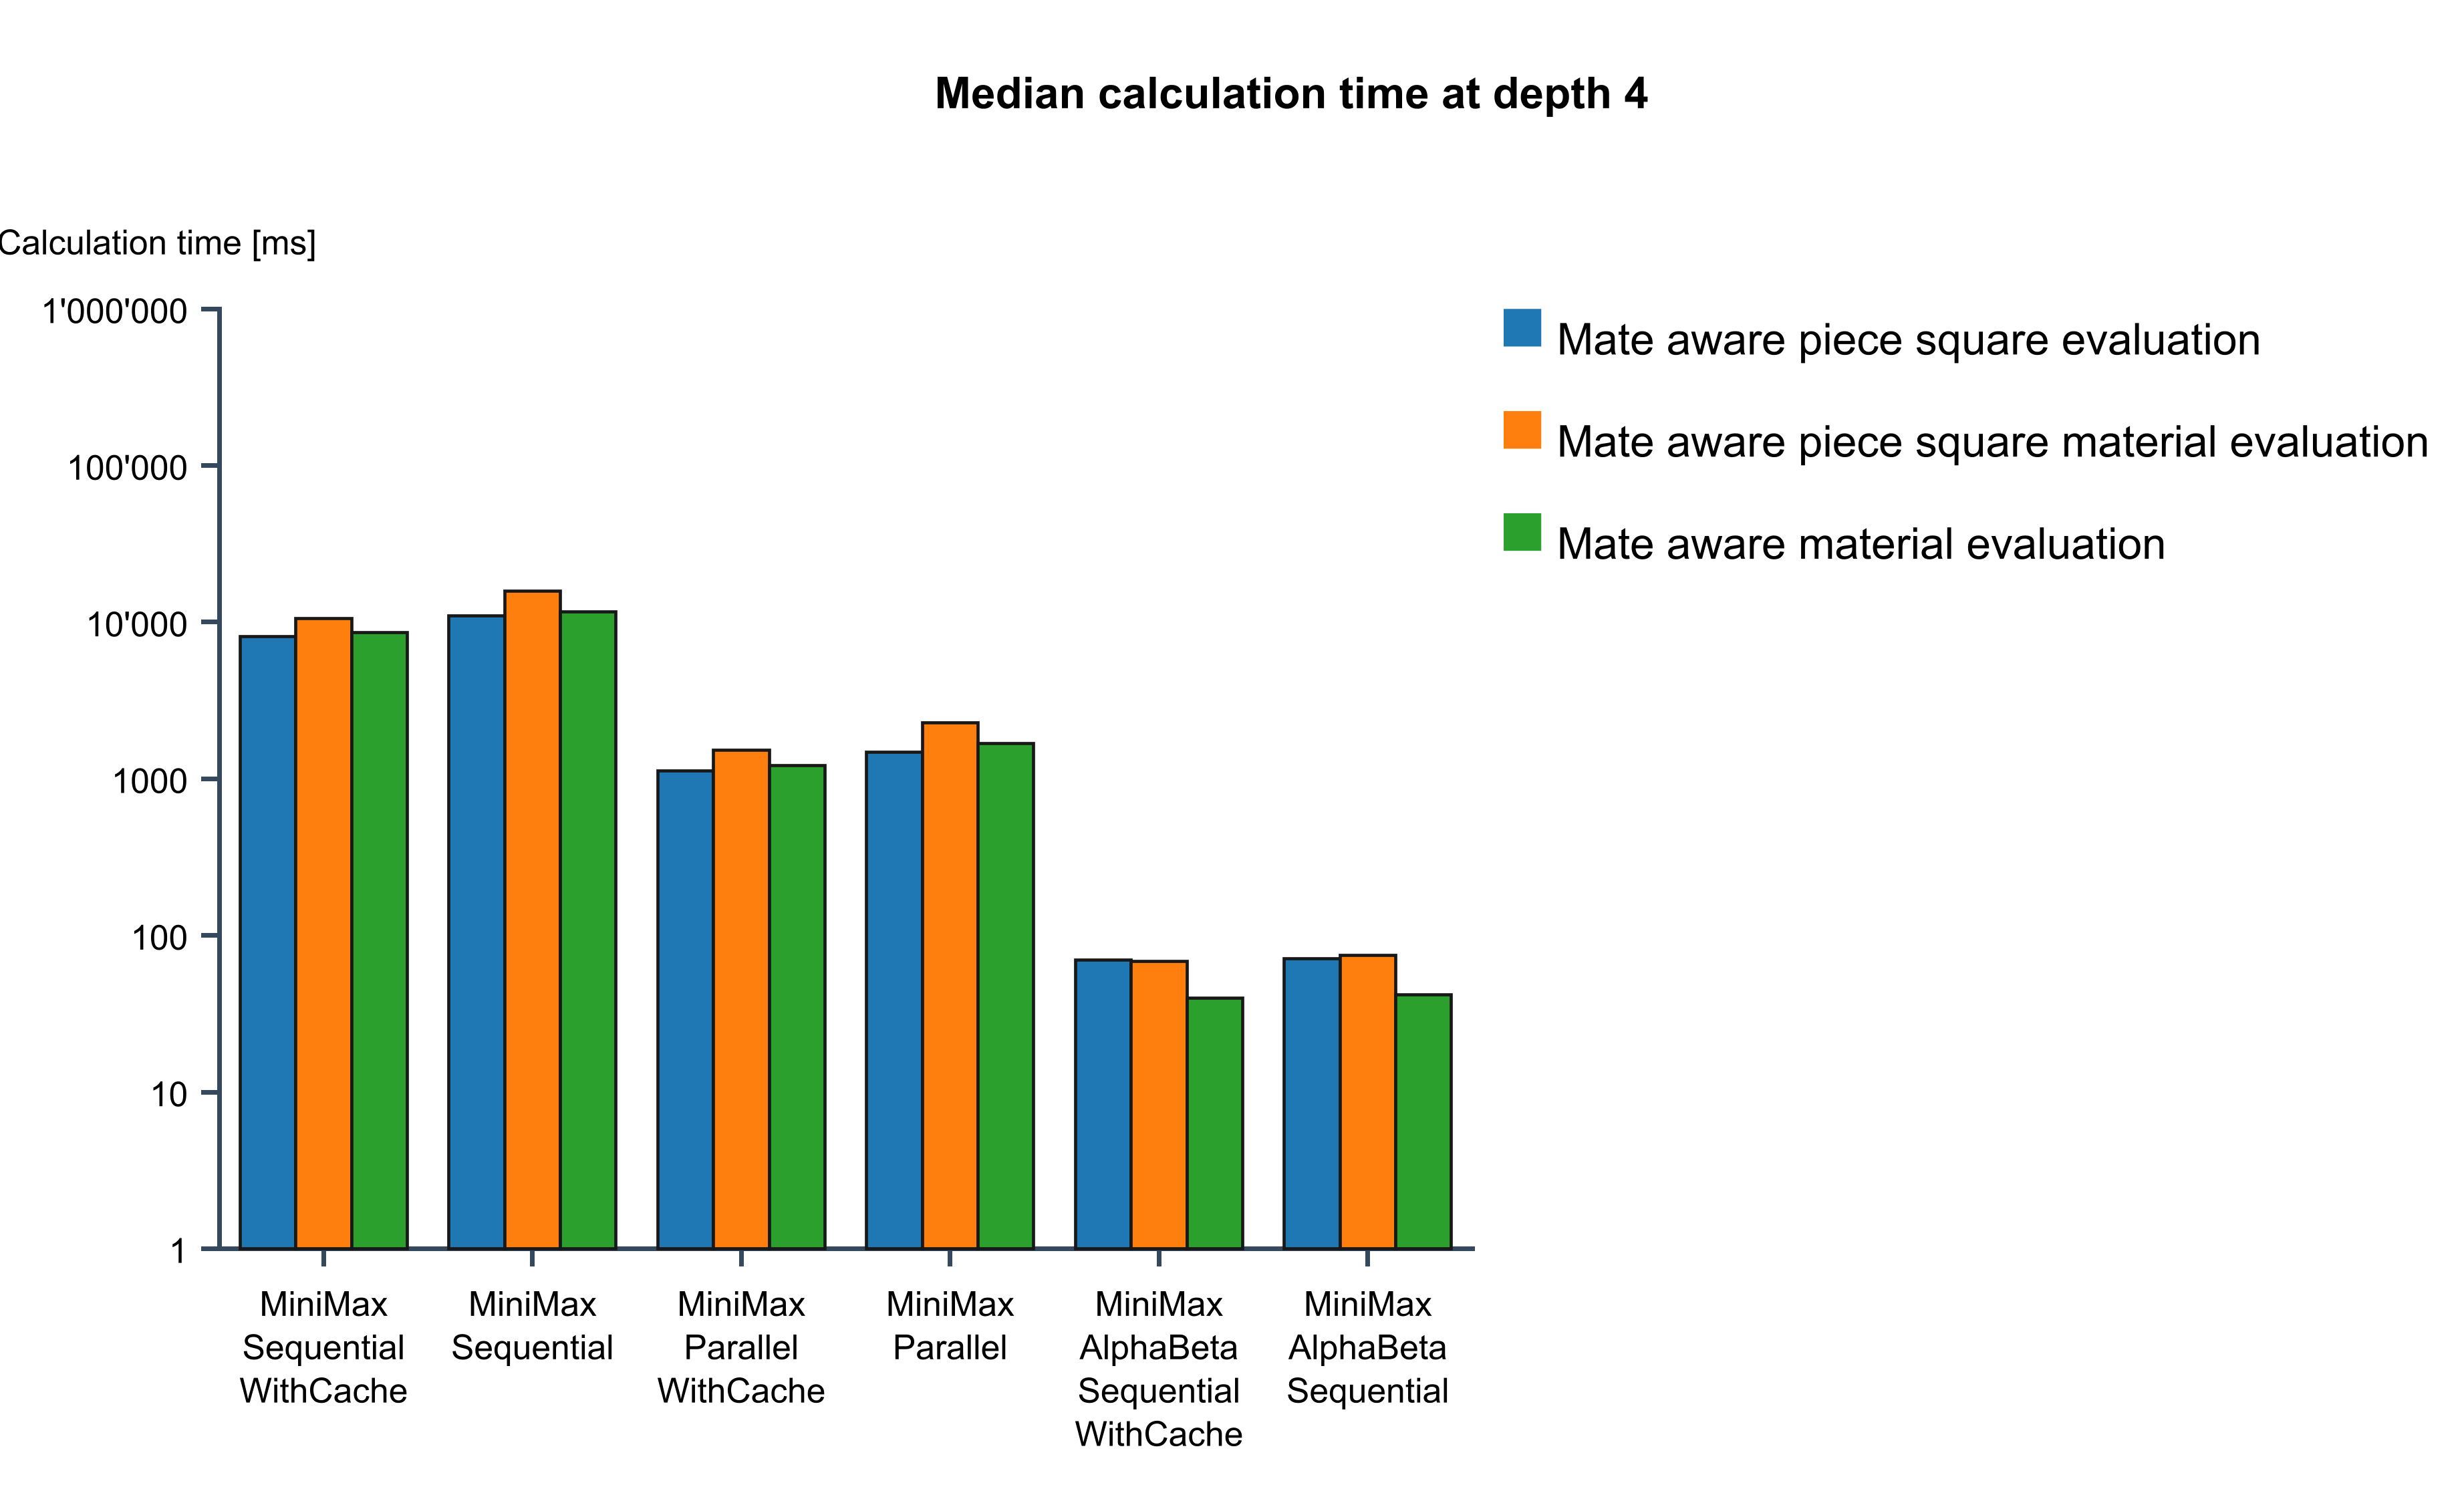
\includegraphics[width=\linewidth]{evaluation/report/performance/performance-at-depth-4-by-strategy}
    \caption{Rechenzeit für Zugtiefe 4}
    \label{fig:rechenzeit-fuer-tiefe-4}
\end{figure}

\begin{figure}[H]
    \centering
    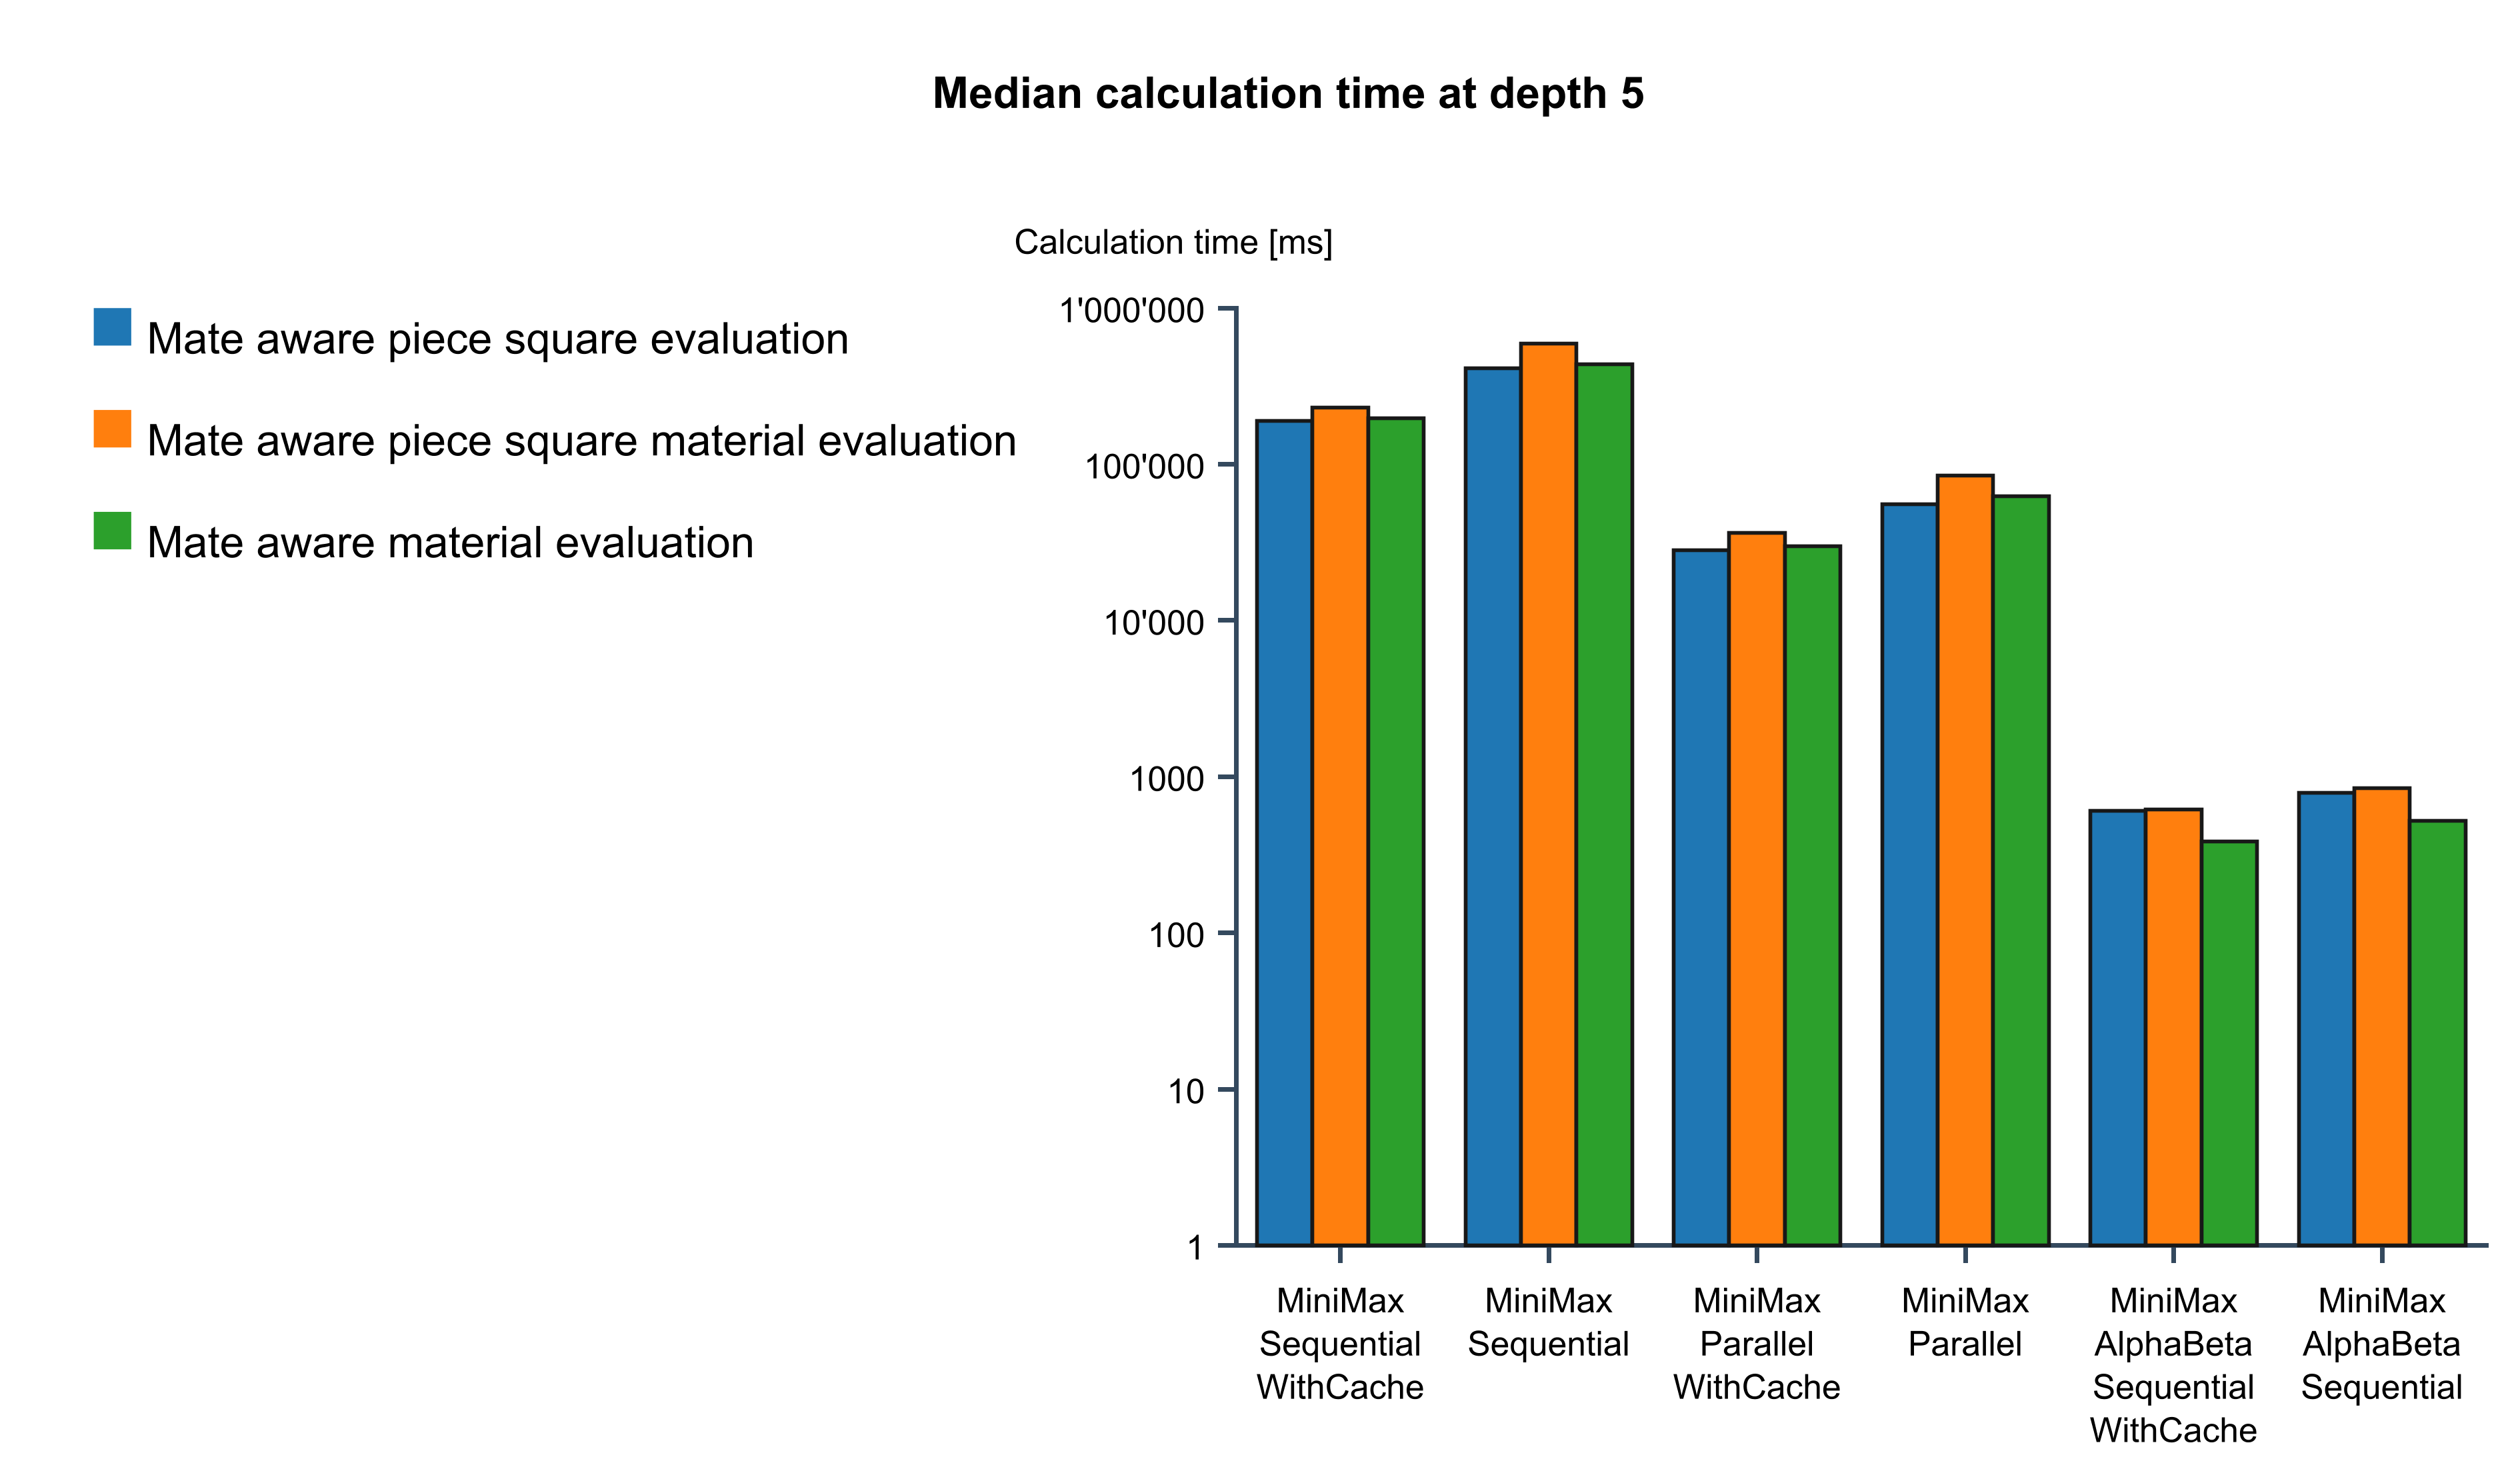
\includegraphics[width=\linewidth]{evaluation/report/performance/performance-at-depth-5-by-strategy}
    \caption{Rechenzeit für Zugtiefe 5}
    \label{fig:rechenzeit-fuer-tiefe-5}
\end{figure}

\begin{figure}[H]
    \centering
    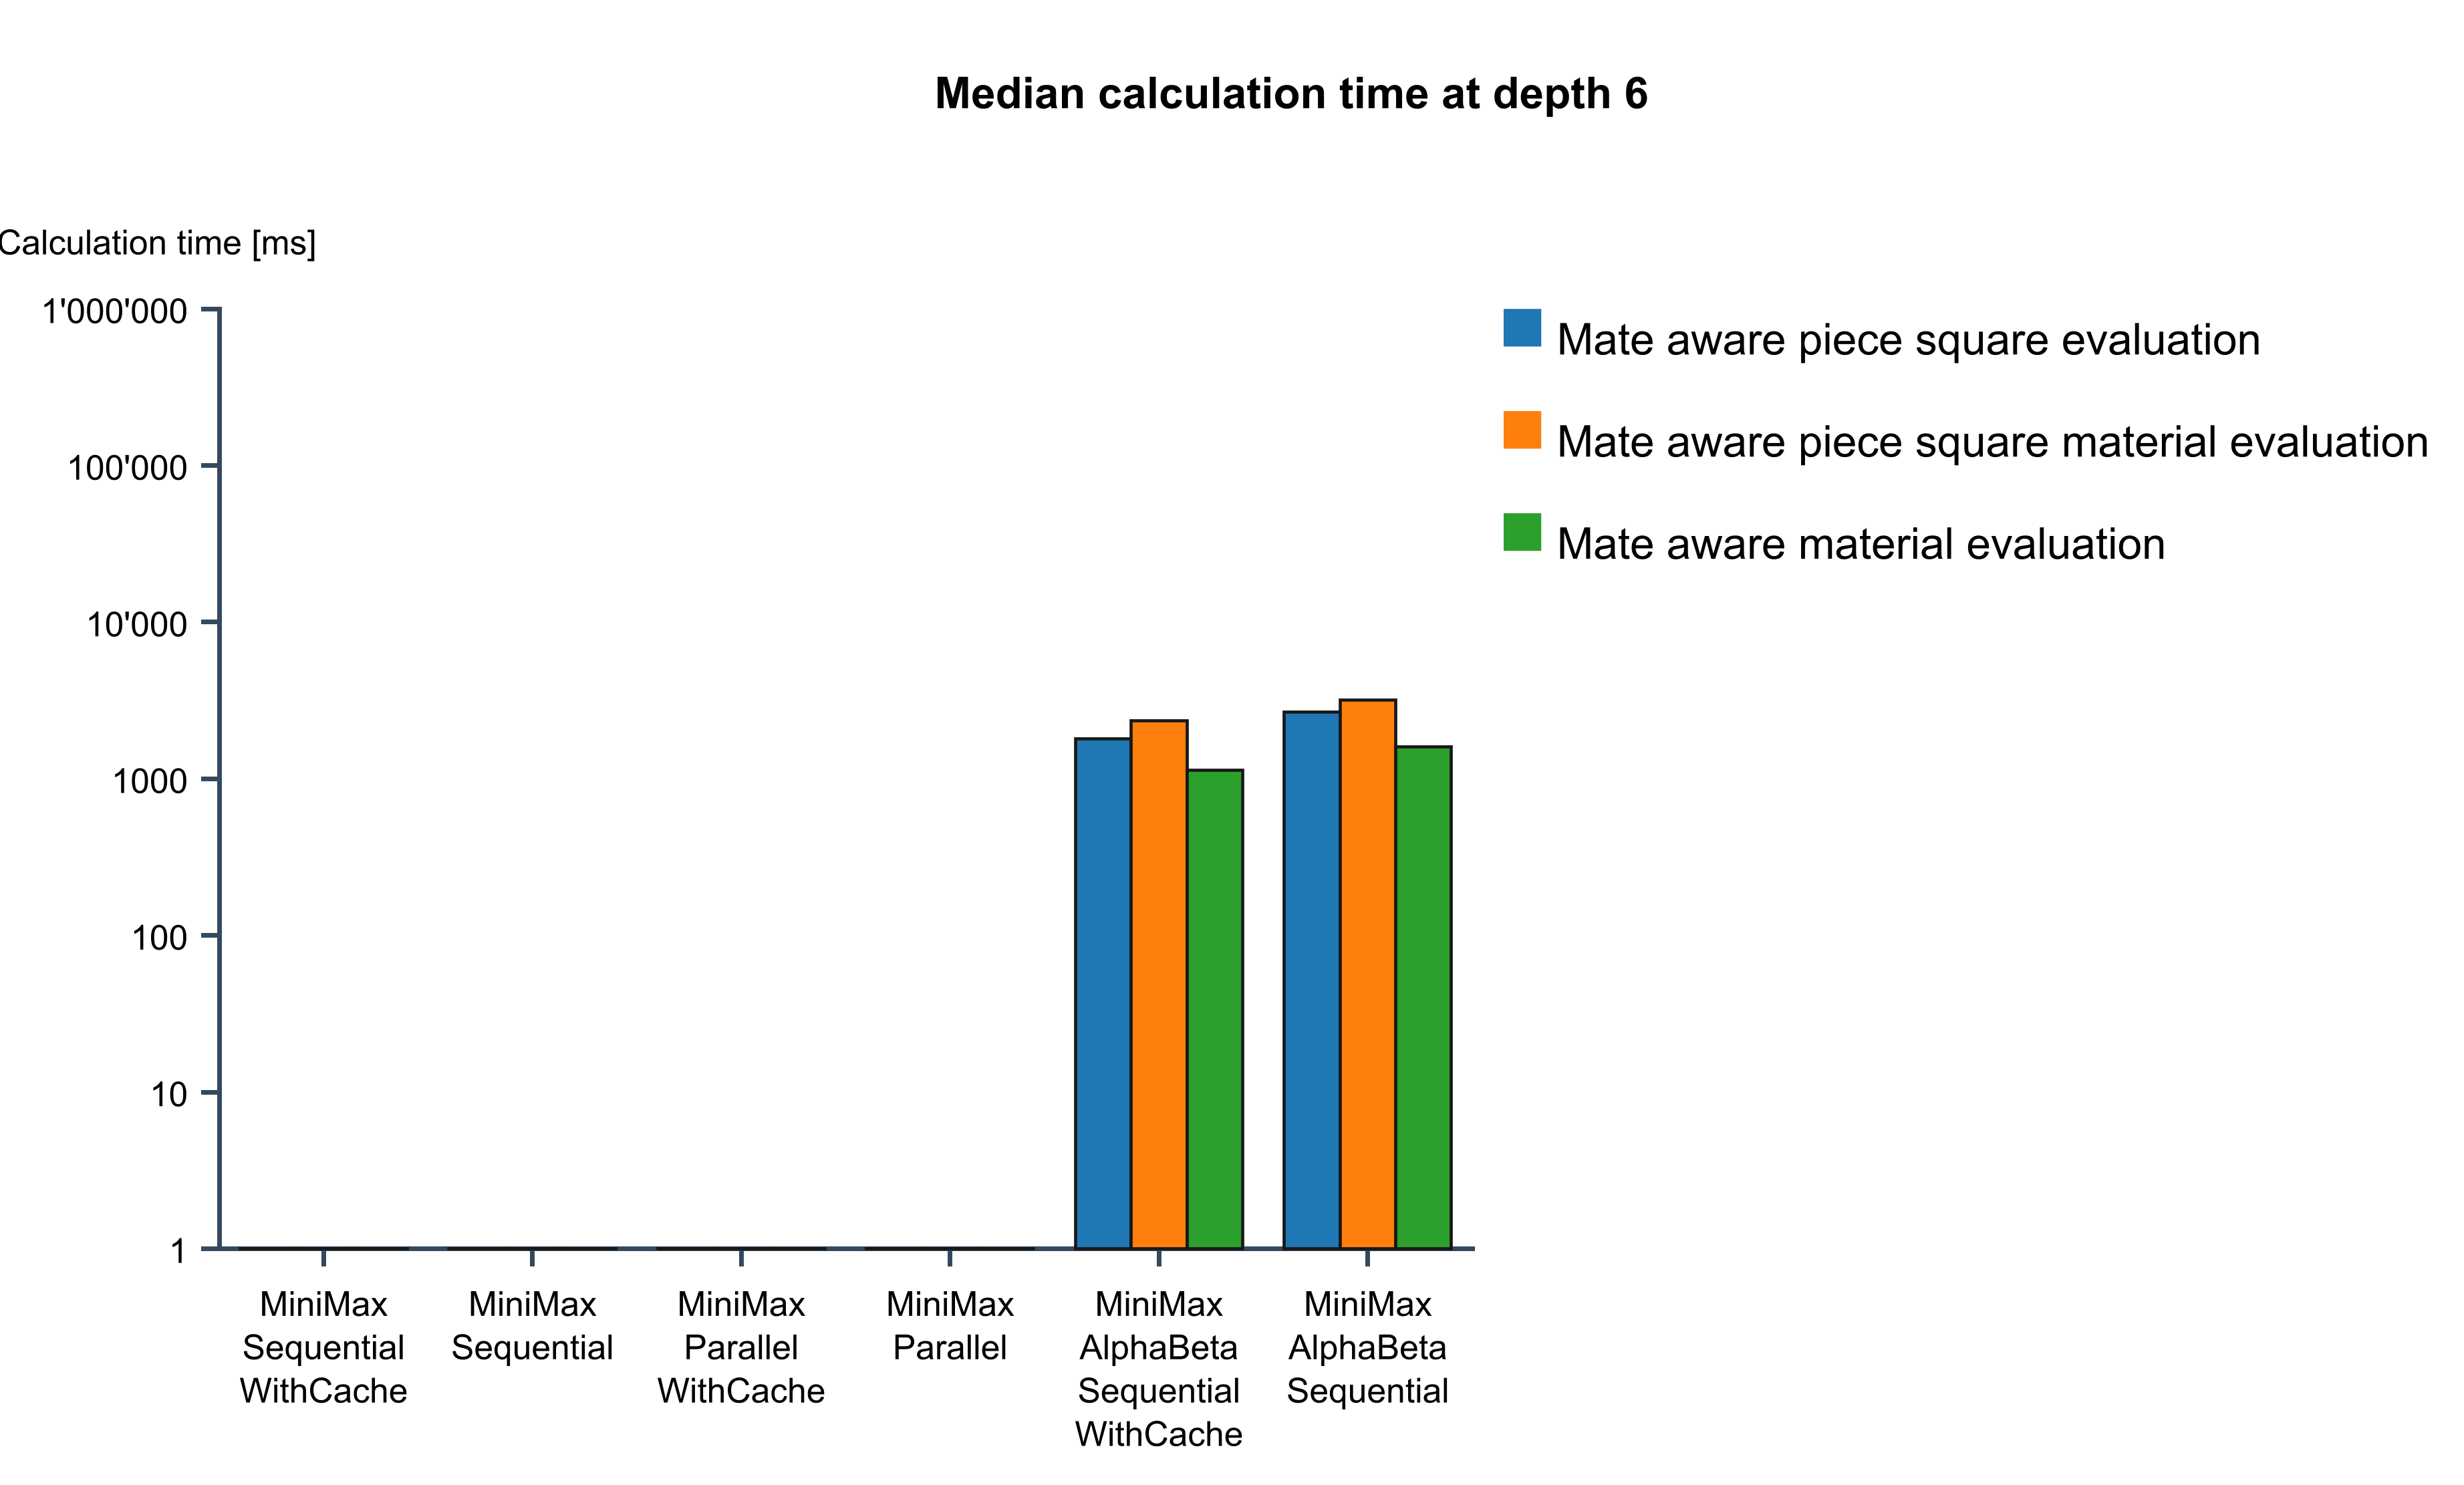
\includegraphics[width=\linewidth]{evaluation/report/performance/performance-at-depth-6-by-strategy}
    \caption{Rechenzeit für Zugtiefe 6}
    \label{fig:rechenzeit-fuer-tiefe-6}
\end{figure}

\begin{figure}[H]
    \centering
    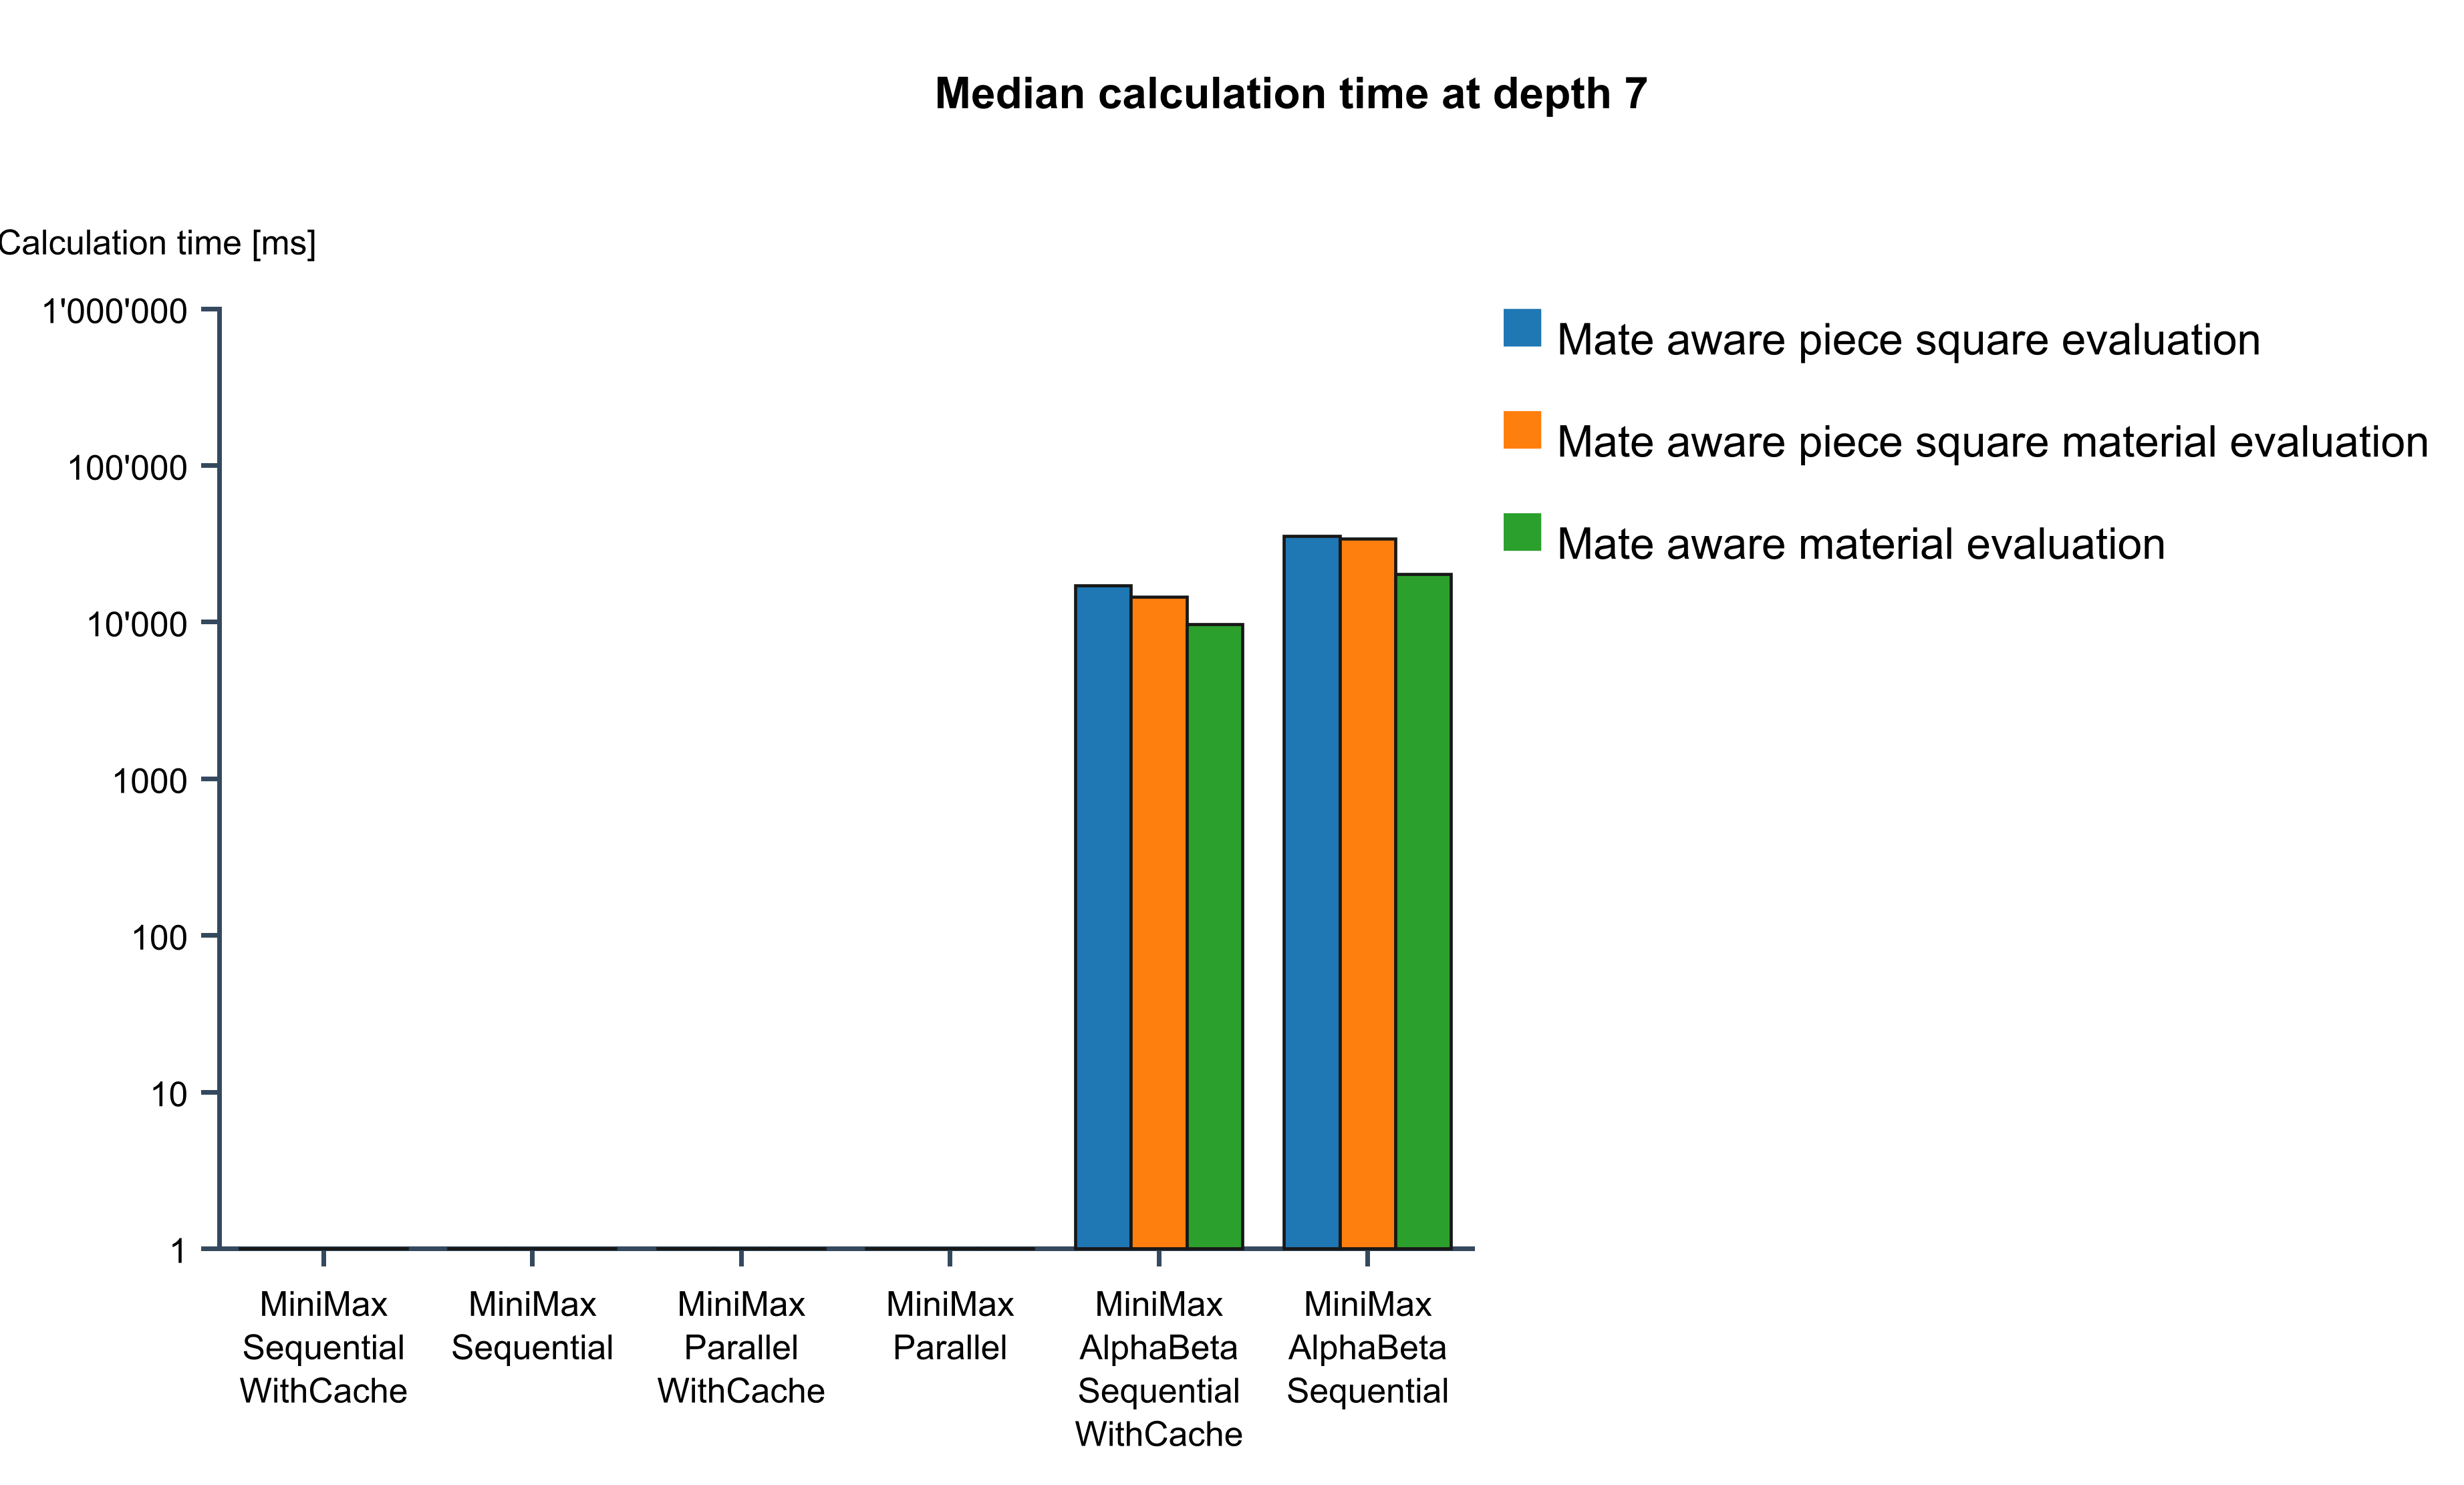
\includegraphics[width=\linewidth]{evaluation/report/performance/performance-at-depth-7-by-strategy}
    \caption{Rechenzeit für Zugtiefe 7}
    \label{fig:rechenzeit-fuer-tiefe-7}
\end{figure}

\newpage
\section{Rechengeschwindigkeitsmultiplikator im Vergleich zu \texorpdfstring{\texttt{MiniMaxSequential}}{MiniMaxSequential}}
\label{sec:performance-gains}
\subfile{evaluation/report/performance/performance-gains-minimaxsequential-at-depth-1-by-position}
\subfile{evaluation/report/performance/performance-gains-minimaxsequential-at-depth-2-by-position}
\subfile{evaluation/report/performance/performance-gains-minimaxsequential-at-depth-3-by-position}
\subfile{evaluation/report/performance/performance-gains-minimaxsequential-at-depth-4-by-position}
\begin{table}[H]
    \centering
    \resizebox{\textwidth}{!}{%
        \input{evaluation/report/performance/performance-gains-minimaxsequential-at-depth-5-by-position}
    }
    \caption{Median performance difference from MiniMaxSequential at depth 5 by position}
    \label{tab:median-performance-difference-from-minimaxsequential-at-depth-5-by-position}
\end{table}

\subfile{evaluation/report/performance/performance-gains-minimaxsequential-at-depth-1-by-strategy}
\subfile{evaluation/report/performance/performance-gains-minimaxsequential-at-depth-2-by-strategy}
\subfile{evaluation/report/performance/performance-gains-minimaxsequential-at-depth-3-by-strategy}
\subfile{evaluation/report/performance/performance-gains-minimaxsequential-at-depth-4-by-strategy}
\begin{table}[H]
    \centering
    \resizebox{\textwidth}{!}{%
        \begin{tabular}{|p{8cm}|*{5}{r|}}
    \hline
    & \multicolumn{5}{c|}{\textbf{Median performance gain multiplier}} \\
    \cline{2-6}
    \multirow{-2}{*}{\parbox{8cm}{\centering\textbf{Strategy}}} & \multicolumn{1}{r|}{\textbf{MiniMaxAlphaBetaSequentialWithCache}} & \multicolumn{1}{r|}{\textbf{MiniMaxAlphaBetaSequential}} & \multicolumn{1}{r|}{\textbf{MiniMaxParallelWithCache}} & \multicolumn{1}{r|}{\textbf{MiniMaxParallel}} & \multicolumn{1}{r|}{\textbf{MiniMaxSequentialWithCache}} \\
    \hline
    \rowcolor[HTML]{FFFFFF}
    \textbf{Mate aware piece square evaluation}                 & 686.42                                                            & 522.20                                                   & 14.67                                                  & 7.44                                          & 2.18                                                     \\

    \rowcolor[HTML]{EFEFEF}
    \textbf{Mate aware piece square material evaluation}        & 955.39                                                            & 699.55                                                   & 16.33                                                  & 7.00                                          & 2.56                                                     \\

    \rowcolor[HTML]{FFFFFF}
    \textbf{Mate aware material evaluation}                     & 1139.56                                                           & 836.50                                                   & 14.74                                                  & 7.01                                          & 2.23                                                     \\
    \hline
    \hline
    \rowcolor[HTML]{FFFFFF}
    \textbf{Median}                                             & \textbf{955.39}                                                   & \textbf{699.55}                                          & \textbf{14.74}                                         & \textbf{7.01}                                 & \textbf{2.23}                                            \\

    \hline
\end{tabular}%

    }
    \caption{Median performance difference from MiniMaxSequential at depth 5 by strategy}
    \label{tab:median-performance-difference-from-minimaxsequential-at-depth-5-by-strategy}
\end{table}